\chapter{Linguaggi e automi a stati finiti}
Nell'ambito generale della diagnosi di sistemi a eventi discreti, il comportamento del sistema è descritto da successioni di eventi. A questo livello di astrazione, il comportamento del sistema è caratterizzato da sequenze di transizioni che possono essere descritte da un automa a stati finiti. Anche il comportamento dei singoli componenti del sistema, come si vedrà in seguito, può essere descritto da un automa. La semplicità e l'intuitività degli automi rende agevole il loro utilizzo in problemi di questo tipo, nonché nella più ampia branca dell'intelligenza artificiale.
Prima dell'esistenza dei calcolatori, negli anni '30, Turing studiò una macchina astratta in grado di poter computare qualsiasi algoritmo. 
Negli anni '40 e '50, numerosi ricercatori hanno studiato tipologie di macchine più semplici, quelle che oggi sono chiamate automi a stati finiti.
Questi automi sono diventati estremamente utili per una grande varietà di scopi, rappresentando modelli per descrivere, ad esempio, molti tipi di hardware e software:
\begin{itemize}
\item software per la progettazione e la verifica del comportamento di circuiti digitali,
\item analizzatori lessicali tipici dei compilatori,
\item software per la scansione di grandi corpi di testo, al fine di trovare parole frasi o altri pattern,
\item software per la verifica di sistemi con un numero finiti di stati distinti, come protocolli di comunicazione o protocolli per lo scambio sicuro di informazioni.
\end{itemize}
Esistono due principali tipi di automi a stati finiti:
\begin{itemize}
\item automi a stati finiti deterministici (DFA);
\item automi a stati finiti non deterministici (NFA).
\end{itemize}
In questo capitolo vengono presentati definizioni, algoritmi ed esempi riguardanti entrambe le classi di automi. In particolare, è descritto come convertire espressioni regolari in NFA e come convertire NFA in DFA.
Da ultimo viene fornito il concetto di automa minimo, cioè un automa caratterizzato dal minor numero di stati possibile, utile per una implementazione efficiente in termini di risorse computazionali.

\newpage
\section{Linguaggi}
Qualsiasi DES possiede un insieme di eventi ad esso associato. Questo insieme può essere visto come l'alfabeto di un linguaggio e le sequenze di eventi generati come parole (o stringhe) appartenenti al linguaggio. Una stringa caratterizzata da nessun simbolo dell'alfabeto è detta stringa vuota e si denota con $\epsilon$.
Data una stringa $s$, la sua lunghezza $|s|$ è il numero di simboli contenuti in essa, tenendo conto di eventuali occorrenze multiple del medesimo simbolo. Per convenzione, la lunghezza della stringa vuota è zero.
\begin{defn}
Un linguaggio definito su un insieme alfabeto $\Sigma$ è un insieme di stringhe di lunghezza finita formate da simboli appartenenti a $\Sigma$.
\end{defn}
L'operazione fondamentale per la costruzione di linguaggi è quella della concatenazione. Se $x$ e $y$ sono stringhe, la loro concatenazione è la stringa $xy$. La stringa vuota è l'elemento identità di tale operazione, poiché per ogni stringa $s$, $s\epsilon = \epsilon s = s$.\\
Un'altra operazione che caratterizza i linguaggi è la chiusura di Kleene, denotata $L^*$, che è l'insieme di tutte le stringhe finite che si ottengono concatenando elementi dell'alfabeto, compresa la stringa vuota.\\
Sui linguaggi è altresì possibile applicare tutte le operazioni insiemistiche quali l'unione, l'intersezione, la differenza e il complemento.
Un linguaggio può essere visto come un modo formale di descrivere il comportamento di un DES, specificando tutte le possibili sequenze di eventi che il sistema è in grado di generare. 
Un automa è un formalismo in grado di rappresentare un linguaggio.
In particolare, nel seguito della trattazione, ci si focalizzerà sui cosiddetti linguaggi regolari, ovvero su quei linguaggi che possono essere rappresentati tramite automi con un numero finito di stati.

\newpage
\section{DFA}
Un automa a stati finiti deterministico (DFA: deterministic finite automaton) è una quintupla:
\begin{center}
	$D = (\Sigma,S,t,s_0,F)$
\end{center}
dove:
\begin{itemize}
\item $\Sigma$ è un alfabeto, ovvero l'insieme dei simboli di input;
\item $S$ è un insieme finito di stati;
\item $t$ è la funzione di transizione (deterministica) $t: S \times \Sigma \rightarrow S$ che associa, ad uno stato e un simbolo di input, un nuovo stato;
\item $s_0$ è lo stato iniziale;
\item $F \subseteq S$ è un insieme di stati finali.
\end{itemize}
Un automa di questo tipo è detto deterministico poiché la sua funzione di transizione non permette l'esistenza, a partire da un medesimo stato, di due transizioni caratterizzate dallo stesso simbolo: l'automa, istantaneamente, si trova in un singolo stato.\\
Esistono due principali rappresentazioni per gli automi:
\begin{itemize}
\item tabella delle transizioni, rappresentazione tabellare della funzione di transizione dove nelle righe si trovano gli stati di partenza, mentre nelle colonne i simboli (o viceversa). L'elemento in una cella della tabella rappresenta lo stato destinazione della transizione, a partire dallo stato della riga corrispondente e in base al simbolo di input nella relativa colonna; particolari notazioni grafiche possono essere utilizzate per contraddistinguere lo stato iniziale e gli stati finali.
\item diagramma delle transizioni, un grafo nel quale:
	\begin{itemize}
	\item ogni stato è rappresentato da un vertice;
	\item ogni transizione è un arco orientato che connette due vertici e possiede una label indicante il simbolo della transizione;
	\item una freccia entrante in un vertice rappresenta lo stato iniziale;
	\item ogni vertice associato ad uno stato finale è descritto da un doppio contorno, mentre gli stati non finali hanno come vertice un contorno singolo.
	\end{itemize}
\end{itemize}

\begin{ex}
Si consideri un DFA con $\Sigma = \{ a,b,c\}$, $S = \{ s_0,s_1,s_2\}$, stato iniziale $s_0$, insieme di stati finali $F = \{s_2\}$ e funzione di transizione $t$ che si evince dalle rappresentazioni in tabella \ref{tab:dfa} e figura \ref{fig:dfa}.
Si noti come la funzione di transizione non debba essere necessariamente completa.

\begin{table}[htbp]
\begin{center}
\begin{tabular}{r | c c c}
& a & b & c \\ \hline
$\rightarrow s_0$ & $s_1$ & $-$ & $s_0$ \\
$s_1$ & $-$ & $s_2$ & $-$\\
$*s_2$ & $-$ & $-$ & $-$\\ 
\end{tabular}
\caption{Rappresentazione tramite tabella di un DFA}
\label{tab:dfa}
\end{center}
\end{table}


\begin{figure}[htbp]
\centering
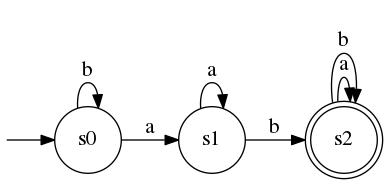
\includegraphics[scale=0.3]{./Img/automi/ex1.png}
\caption{Rappresentazione grafica di un DFA}
\label{fig:dfa}
\end{figure}

\end{ex}

\newpage
\section{NFA}
Un automa finito non deterministico (NFA: nondeterministic finite automaton) è, similmente ad un DFA, una quintupla:
\begin{center}
	$N = (\Sigma,S,t,s_0,F)$
\end{center}
dove:
\begin{itemize}
\item $\Sigma$ è un alfabeto, ovvero l'insieme dei simboli di input;
\item $S$ è un insieme finito di stati;
\item $t$ è la funzione di transizione (non deterministica) $t: S \times (\Sigma \cup \{\epsilon\}) \rightarrow 2^S$ che associa, ad uno stato e un simbolo di input (oppure al simbolo vuoto $\epsilon$), un insieme di stati;
\item $s_0$ è lo stato iniziale;
\item $F \subseteq S$ è un insieme di stati finali.
\end{itemize}
La differenza tra gli automi deterministici e quelli non deterministici riguarda la funzione di transizione, che in quest'ultima classe di automi presenta due forme di non determinismo: da un lato, la presenza di $\epsilon$-transition possono cambiare lo stato corrente dell'automa senza che venga consumato alcun simbolo in input; d'altro canto, la possibile presenza di transizione uscenti dal medesimo stato con la stessa label fornisce una scelta non deterministica nella percorrenza dell'automa.
Il teorema che è analizzato nella sezione successiva mostra che è sempre possibile, partendo da un NFA, ricostruire un corrispondente DFA equivalente.
L'utilizzo di automi non deterministici è dettato dalla maggior facilità di modellazione nell'ambito di alcuni algoritmi specifici, nonché da procedure note che permettono di costruire un automa non deterministico equivalente ad una espressione regolare data \footnote{Si noti che, come presentato in \cite{book:compilers}, è altresì possibile costruire direttamente, partendo da un'espressione regolare, un DFA.}.\\
Le possibili rappresentazioni di NFA sono simili a quelle viste per i DFA, con piccole variazioni: nella rappresentazione tabellare ogni cella, invece che contenere un singolo stato, racchiude un insieme di stati, e come simboli si aggiunge una colonna che esplicita le transizioni scatenate dal simbolo vuoto; nella rappresentazione grafica, si ricorre a frecce con la label $\epsilon$ per indicare le $\epsilon$-transition.

\begin{ex}
Viene di seguito riportato un esempio di NFA.
\end{ex}

\newpage
\section{Subset construction}
A causa del loro non determinismo, spesso i NFA necessitano di essere convertiti in DFA per essere utilizzati e simulati in maniera efficiente. La tecnica nota in letteratura per ottenere questa conversione è chiamata subset construction.
L'idea generale di questo algoritmo è che ad ogni stato del risultante DFA corrisponde un insieme di stati del NFA di partenza.
\'E possibile, teoricamente, che il numero di stati del DFA sia esponenziale nel numero di stati del NFA: tale numero è limitato superiormente dalla cardinalità dell'insieme potenza degli stati dell'automa non deterministico, cioè dal numero di tutti i possibili sottoinsiemi degli stati.
Fortunatamente, questo caso pessimo raramente si presenta e per linguaggi reali spesso il numero di stati dei due automi è simile e il comportamento esponenziale non sussiste.\\
Il primo problema che bisogna affrontare è quello di gestire le $\epsilon$-transition. Queste particolari transizioni indicano in quali stati l'automa può trovarsi contemporaneamente. L'operazione di $\epsilon$-chiusura permette di trovare, a partire da un particolare stato, tutti gli stati raggiungibili senza la consumazione di simboli in ingresso. Il primo passo della subset construction, quindi, consiste nell'assegnare allo stato iniziale del DFA risultante la $\epsilon$-chiusura dello stato iniziale del NFA in esame. L'algoritmo prosegue calcolando, per ogni possibile input ricevuto in ogni stato del NFA appartenente allo stato iniziale del risultato, l'insieme degli stati raggiungibili, su cui viene effettuata la $\epsilon$-chiusura. Il procedimento procede in questo modo sino a che tutti i nuovi stati generati del DFA non sono stati processati.

\newpage
\section{Espressioni regolari}
Le espressioni regolari costituiscono quell'insieme di linguaggi che possono essere rappresentati da automi a stati finiti (grammatica di tipo 3 della gerarchia di Chomsky). Le espressioni regolari descrivono tutti i linguaggi che possono essere costruiti applicando ai simboli appartenenti ad un alfabeto $\Sigma$ gli operatori di unione, concatenazione e chiusura. Le espressioni regolari sono generate ricorsivamente dalle sottoespressioni che le formano, secondo le seguenti regole.
\begin{enumerate}
\item $\epsilon$ è una espressione regolare che denota il linguaggio $L(\epsilon) = \{\epsilon\}$, 					contenente la sola stringa vuota;
\item se $a$  è un simbolo in $\Sigma$, allora $a$ è un'espressione regolare che denota il linguaggio $L(a) = 	\{a\}$, contenente la sola stringa di lunghezza unitaria $a$.
\item se $x$ e $y$ sono espressioni regolari che denotano rispettivamente i linguaggi $L(x)$ e $L(y)$, allora:
	\begin{itemize}
	\item $(x)$ è l'espressione regolare che denota il linguaggio $L(x)$;
	\item $(x) | (y)$ è l'espressione regolare che denota il linguaggio $L(x) \cup L(y)$ (unione);
	\item $(x)(y)$ è l'espressione regolare che denota il linguaggio $L(x)L(y) = \{xy | x \in L(x), y \in L(y)\}$ (concatenazione);
	\item $(x)^*$ è l'espressione regolare che denota il linguaggio $(L(x))^*$: ripetizione zero o più volte di stringhe in $L(x)$ (chiusura di Kleene).
	\end{itemize}
\end{enumerate}
Altri operatori possono essere definiti opportunamente in base al dominio applicativo, generando espressioni regolari estese.

\newpage
\subsection{Costruzione di Thompson}
La costruzione di McNaughton-Yamada-Thompson (o costruzione di Thompson) è in grado di convertire una qualsiasi espressione regolare in un NFA caratterizzato dal medesimo linguaggio. L'algoritmo opera scomponendo l'espressione regolare in un albero sintattico e costruendo un NFA per ogni sottoespressione, in maniera bottom-up, utilizzando le $\epsilon$-transition come "collante" per unire i sottoautomi. L'automa risultante permette di riconoscere se una stringa appartiene o meno al linguaggio relativo all'espressione regolare di partenza.\\
Le regole viste in precedenza generano dei sottoautomi come schematizzato nelle figure \ref{fig:re_atom}, \ref{fig:re_union}, \ref{fig:re_concat} e \ref{fig:re_closure}. In particolare, il primo diagramma corrisponde alle prime due regole di base della costruzione di espressioni regolari, mentre gli altri tre costituiscono le cosiddette regole induttive, che permettono di generare l'automa completo in maniera incrementale.

\begin{figure}[htbp]
\centering
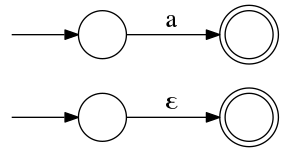
\includegraphics[scale=0.4]{./Img/automi/re_atom.png}
\caption{NFA per espressioni regolari atomiche}
\label{fig:re_atom}
\end{figure}


\begin{figure}[htbp]
\centering
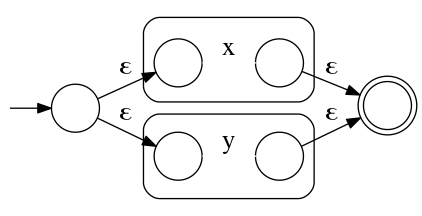
\includegraphics[scale=0.4]{./Img/automi/re_union.png}
\caption{NFA per l'unione di due espressioni regolari}
\label{fig:re_union}
\end{figure}

\begin{figure}[htbp]
\centering
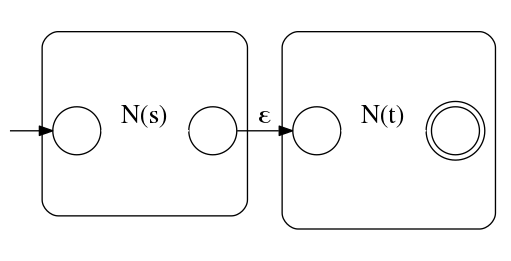
\includegraphics[scale=0.4]{./Img/automi/re_concat.png}
\caption{NFA per la concatenazione di due espressioni regolari}
\label{fig:re_concat}
\end{figure}

\begin{figure}[htbp]
\centering
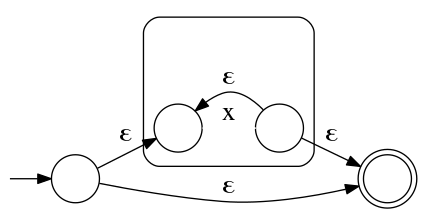
\includegraphics[scale=0.4]{./Img/automi/re_closure.png}
\caption{NFA per la chiusura di un'espressione regolare}
\label{fig:re_closure}
\end{figure}


\newpage
\section{Minimizzazione degli stati}
Dato un linguaggio, possono esistere più automi deterministici che lo riconoscono. Si cerca sempre di scegliere l'automa che presenta il minor numero di stati, dato che l'implementazione di quest'ultimo consente di risparmiare memoria e tempo nella simulazione. 
Esiste sempre un unico DFA minimo per ogni linguaggio regolare, a meno di una ridenominazione del nome degli stati. Questo particolare automa può essere costruito raggruppando insieme quegli stati che sono tra loro equivalenti. Per capire come verificare tale equivalenza, si ricorre al concetto di distinguibilità.
\begin{defn}
La stringa $x$ distingue lo stato $s$ dallo stato $t$ se esattamente uno degli stati raggiunti partendo da $s$ e da $t$ seguendo il cammino con label $x$ è uno stato finale. Quindi, lo stato $s$ è distinguibile dallo stato $t$ se esiste una stringa che li distingue.
In particolare, la stringa vuota distingue ogni stato finale da qualsiasi stato non finale.
\end{defn}

L'algoritmo di minimizzazione degli stati funziona partizionando gli stati dell'automa in gruppi di stati indistinguibili. 
In ogni istante, l'algoritmo mantiene partizioni di stati che non sono ancora stati distinti.
Inizialmente gli stati sono divisi in due macro-partizioni, una contenente gli stati non finali, l'altra contente quelli finali. La divisione iniziale viene raffinata individuando un simbolo di input che distingue tra loro alcuni degli stati appartenenti ad un gruppo, generando in questo modo una ulteriore suddivisione interna. La procedura viene applicata fino a quando nessun gruppo, per ogni simbolo di input, può essere scisso nuovamente.
Infine ogni gruppo di stati, scegliendo per ogni insieme uno stato come rappresentante, viene fuso in un singolo stato che appartiene all'automa minimo risultante. 
